 
\chapter{Surface Tension}

\subsection{Height Function}

The height function is calculated as shown in Fig. \ref{height_function} (when absoulute value of y-normal of interface is greater
than x-normal), as
\begin{enumerate}
 \item Start the summation from the middle row
 \item Sum upwards as long as the cells contain dark fluid
 \item Sum downwards as long as the cells contain light fluid,
but subtract one for each cell added
\item The sums result in a histogram which approximates the
interface
\end{enumerate}



The radius of curvature is given by,
\begin{equation}
 \kappa = -\frac{h^{''}(x)}{[1+(h^{'}(x))^2]^{3/_2}}	%{h^{''}(x)} {[1+(h^'(x))^2]^{3/_2}}
\end{equation}


\begin{figure}
 \centering
 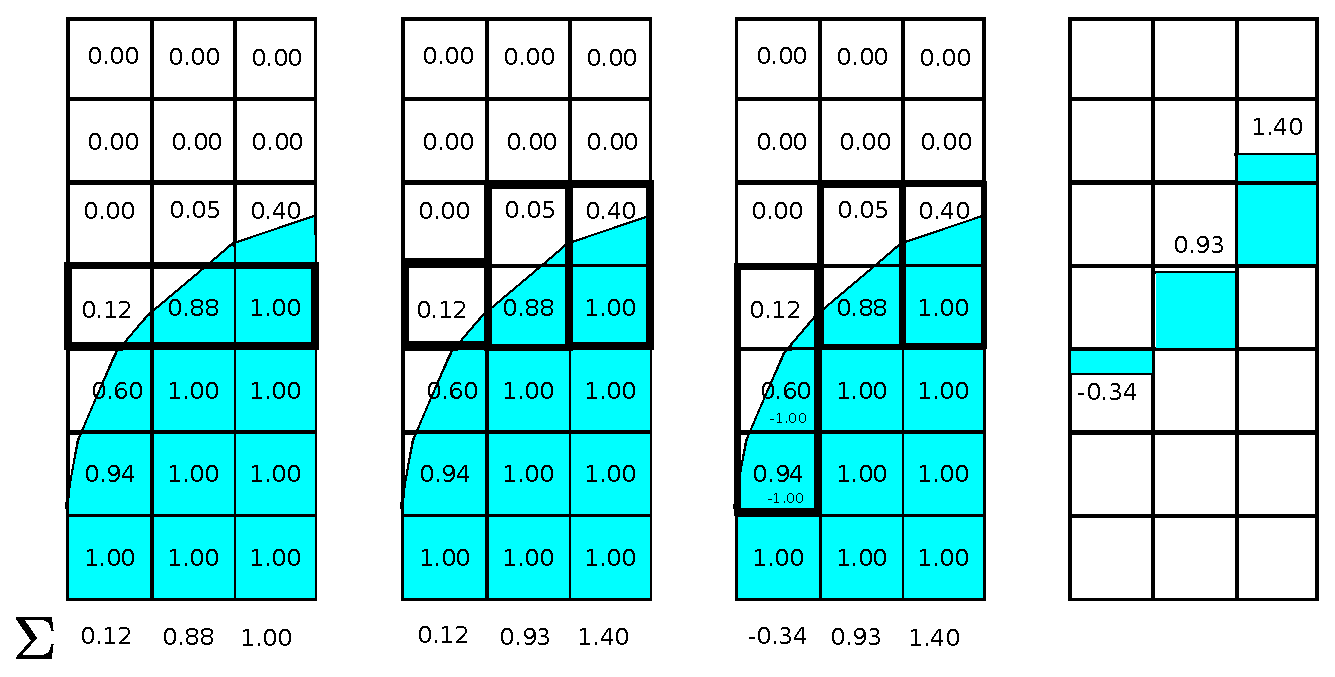
\includegraphics[scale=0.6]{height_function.eps}
 \caption{Variable Stencil for calculation of height functions}
 \label{height_function}
\end{figure}

\begin{algorithm}
  \caption{Height Function algorithm}\label{euclid}
  \begin{algorithmic}[1]
    \Procedure{Height}{$F$}\Comment{Volume Fractions as argument}
%       \State $r\gets a\bmod b$
%       \While{$r\not=0$}\Comment{We have the answer if r is 0}
%         \State $a\gets b$
%         \State $b\gets r$
%         \State $r\gets a\bmod b$
%       \EndWhile\label{euclidendwhile}
      \For{\texttt{Traverse through all cells}}
        \State \If{$0<F<1$} \Comment{if cell contains the interface}
        \State $d = max(|nx|,|ny|)$ \Comment {find the direction of maximum normal}
        \State \While {$F>0$} %\Comment{Sum in d direction as long as the cells contain dark fluid}
        \State \texttt{$H = \sum_d F_d$}
        \State $d=d+1$
        \EndWhile
         \State \While {$F>0$} %\Comment{Sum in negative-d direction as long as the cells contain light fluid}
        \State \texttt{$H = \sum_d (F-1)$}
         \State $d=d-1$
        \EndWhile
	 \State \EndIf 
      \EndFor
      \State \textbf{return} $H$\Comment{The Height Function is $H$}
    \EndProcedure
  \end{algorithmic}
\end{algorithm}


\setlength\tabcolsep{1mm}

\begin{table}[t]
  \begin{center}
    \caption{Comparison of spurious currents, The capillary number is computed by different surface tension methods}
    \label{table:bp}
      \begin{tabular}{c c c c c c c c c c}
	\toprule
	Case & $La$ & $\frac{\rho_{liq}}{\rho_{gas}}$ & $\frac{\mu_{liq}}{\mu_{gas}}$ & $\frac{D}{h}$ & CSS & CSF & FT & CSF\footnote{*Present Study} & HF\footnote{ Present Study} \\
	\midrule
	A & 0.357 & 1 & 1 & 32 	& $3x10^{-3}$ & $1.2x10^{-2}$ & $3.0x10^{-4}$ & $1.22x10^{-2}$ & NA \\
	B & $2x10^{6}$ & 1 & 1 & 32 & $3x10^{-4}$ & $5.0x10^{-4}$ & $1.5x10^{-4}$ & disintegrates & NA \\
	C & $2x10^{6}$ & $10^3$ & 1 & 32 & disintegrates & $3.5x10^{-3}$ & $1.1x10^{-3}$ & $1.5x10^{-3}$ & NA \\
	D & $2x10^{6}$ & $10^3$ & 50 & 32 & disintegrates & $4.5x10^{-3}$ & blows up & $1.6x10^{-3}$ & NA \\ 
	\bottomrule
      \end{tabular}
    \end{center}
 \end{table}
 
  \begin{figure}
 \centering
 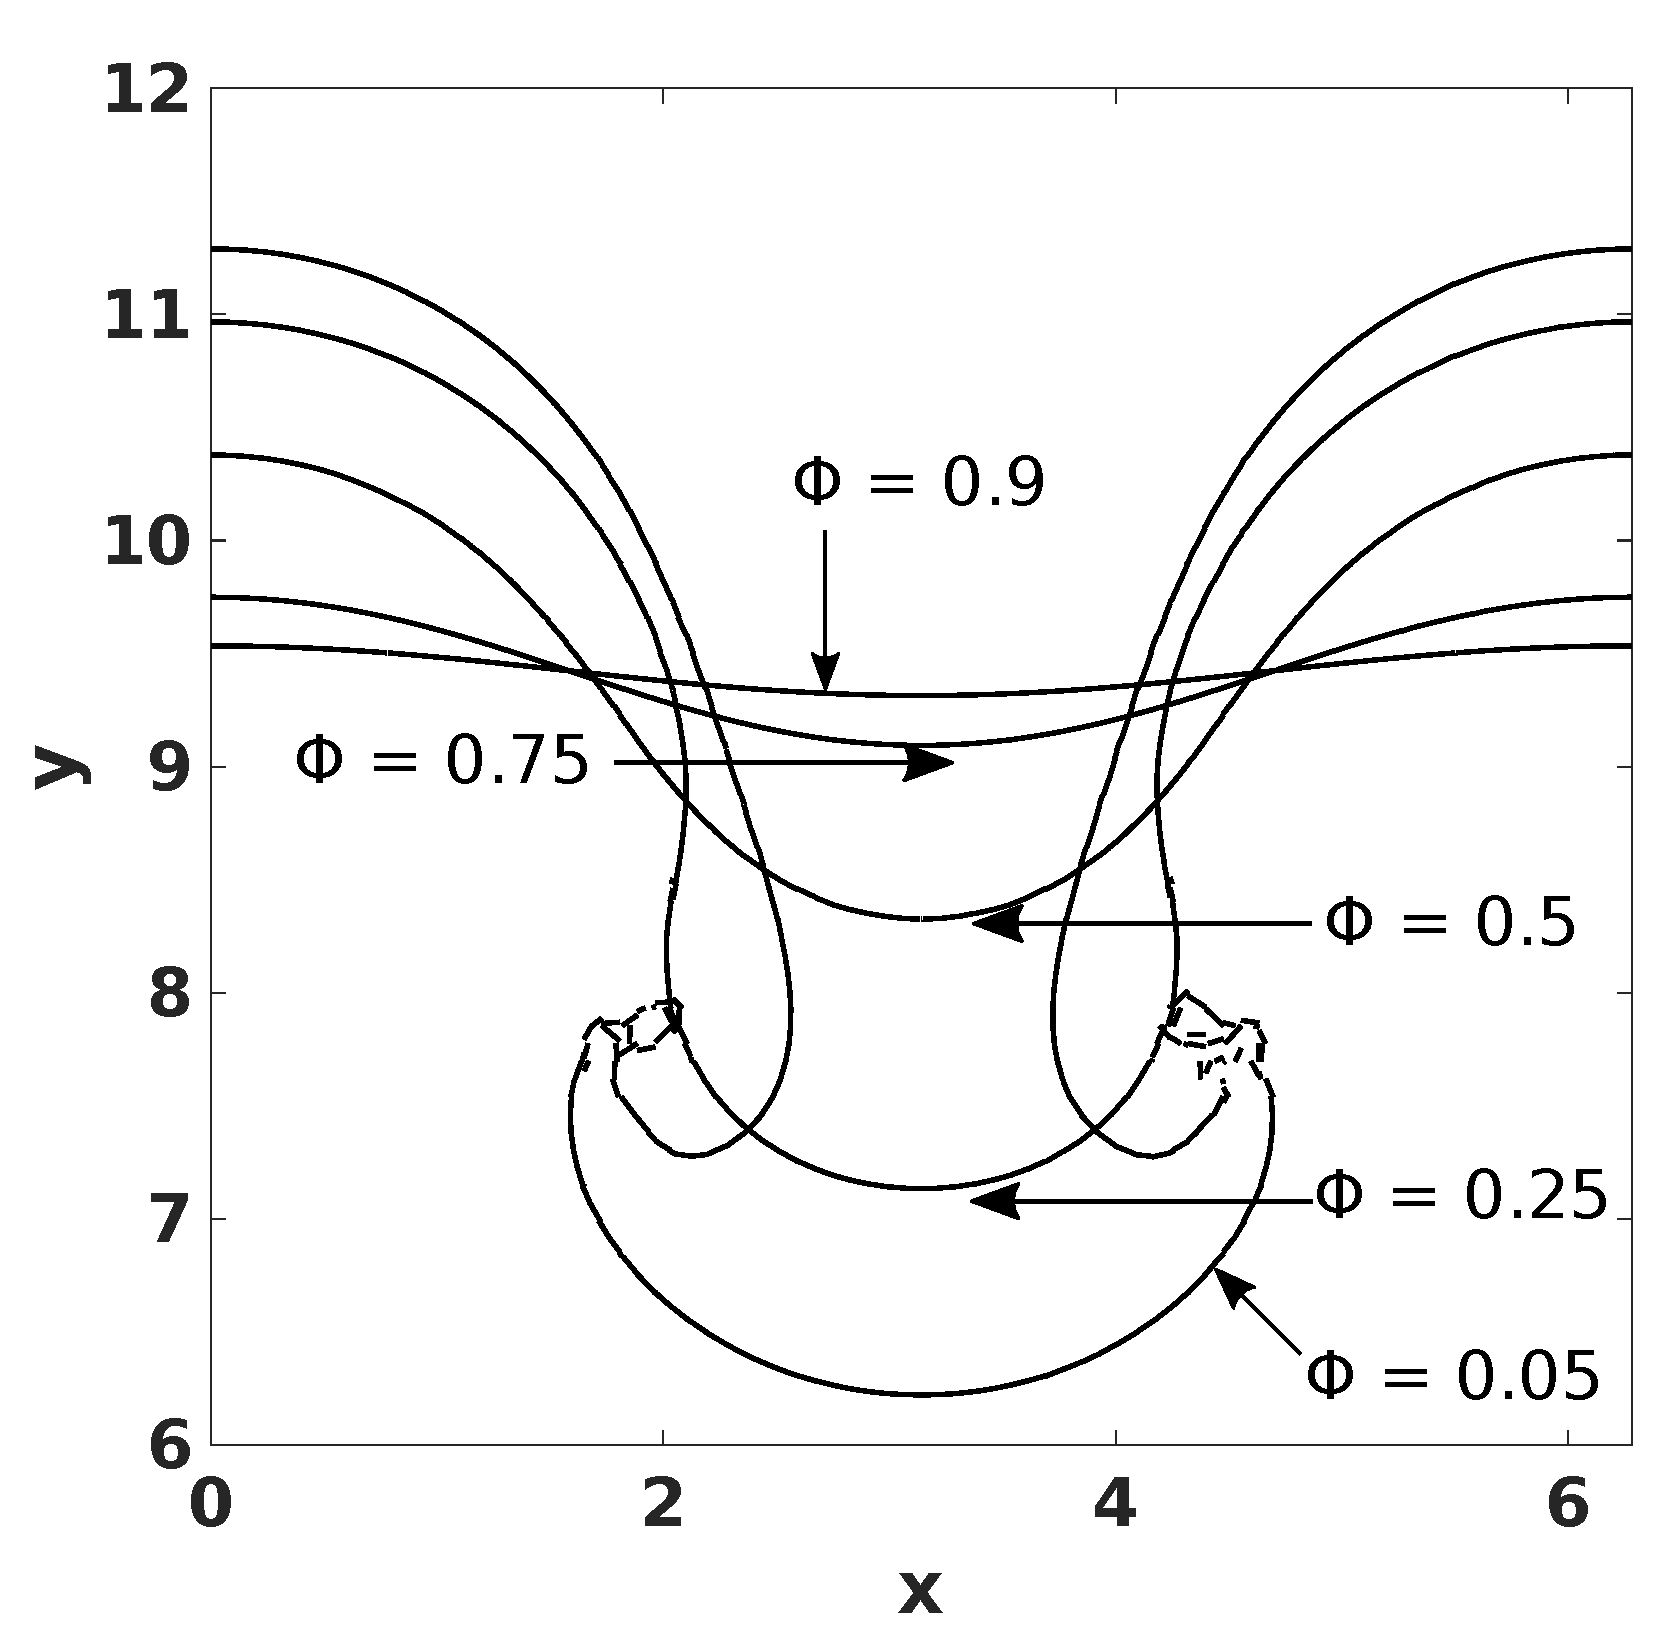
\includegraphics[scale=0.4]{interfaces_diff_phi.eps}
 \caption{Interface shapes for different values of $\Phi$ using Height Function at $\tau = 6$}
\end{figure}
 
\begin{table}[t]
  \begin{center}
    \caption{Comparison of growth rate n among the various numerical methods(PROST, CLSVOF, $K_8$ and HF) and analytical results with
    respect to relative importance of surface tension $\Phi$}
    \label{table:bp}
      \begin{tabular}{c c c c c c c}
	\toprule
	Method & Grid & $\Phi=0.05$ &  $\Phi=0.25$ &  $\Phi=0.5$ &  $\Phi=0.75$ &  $\Phi=0.9$ \\
	\midrule
	PROST &  20 x 60 & 5.7\% & 6.2\% & 6.1\% & 6.0\% & 3.5\% \\
	      &  40 x 120 & 2.3\% & 2.4\% & 2.7\% & 2.7\% & 0.9\% \\
	      &  80 x 240 & 1.0\% & 1.0\% & 0.9\% & 1.9\% & 0.9\% \\
	      \\
	CLSVOF &   20 x 60 & 7.4\% & 7.7\% & 8.5\% & 10.1\% & 15.3\% \\
	      &  40 x 120 & 2.7\% & 3.4\% & 4.4\% & 5.2\% & 7.5\% \\
	      &  80 x 240 & 0.8\% & 1.5\% & 2.1\% & 2.7\% & 3.5\% \\
	      \\
	$K_8$  &  20 x 60 & 8.7\% & 8.1\% & 9.1\% & 1.4\% & 26.0\% \\
	      &  40 x 120 & 3.6\% & 3.4\% & 3.8\% & 2.2\% & 26.0\% \\
	      &  80 x 240 & 1.5\% & 1.0\% & 2.1\% & 3.0\% & 29.0\% \\
	      \\
	HF    &  20 x 60 & 5.7\% & 6.2\% & 6.1\% & 6.0\% & 3.5\% \\
	      &  40 x 120 & 2.3\% & 2.4\% & 2.7\% & 2.7\% & 0.9\% \\
	      &  80 x 240 & 1.0\% & 1.0\% & 0.9\% & 1.9\% & 0.9\% \\
	      \\
	Exact n	& 	  & 2.365 & 2.101 & 1.716 & 1.213 & 0.767 	\\
	\bottomrule
      \end{tabular}
    \end{center}
 \end{table}
 
 \begin{figure}
 \centering
 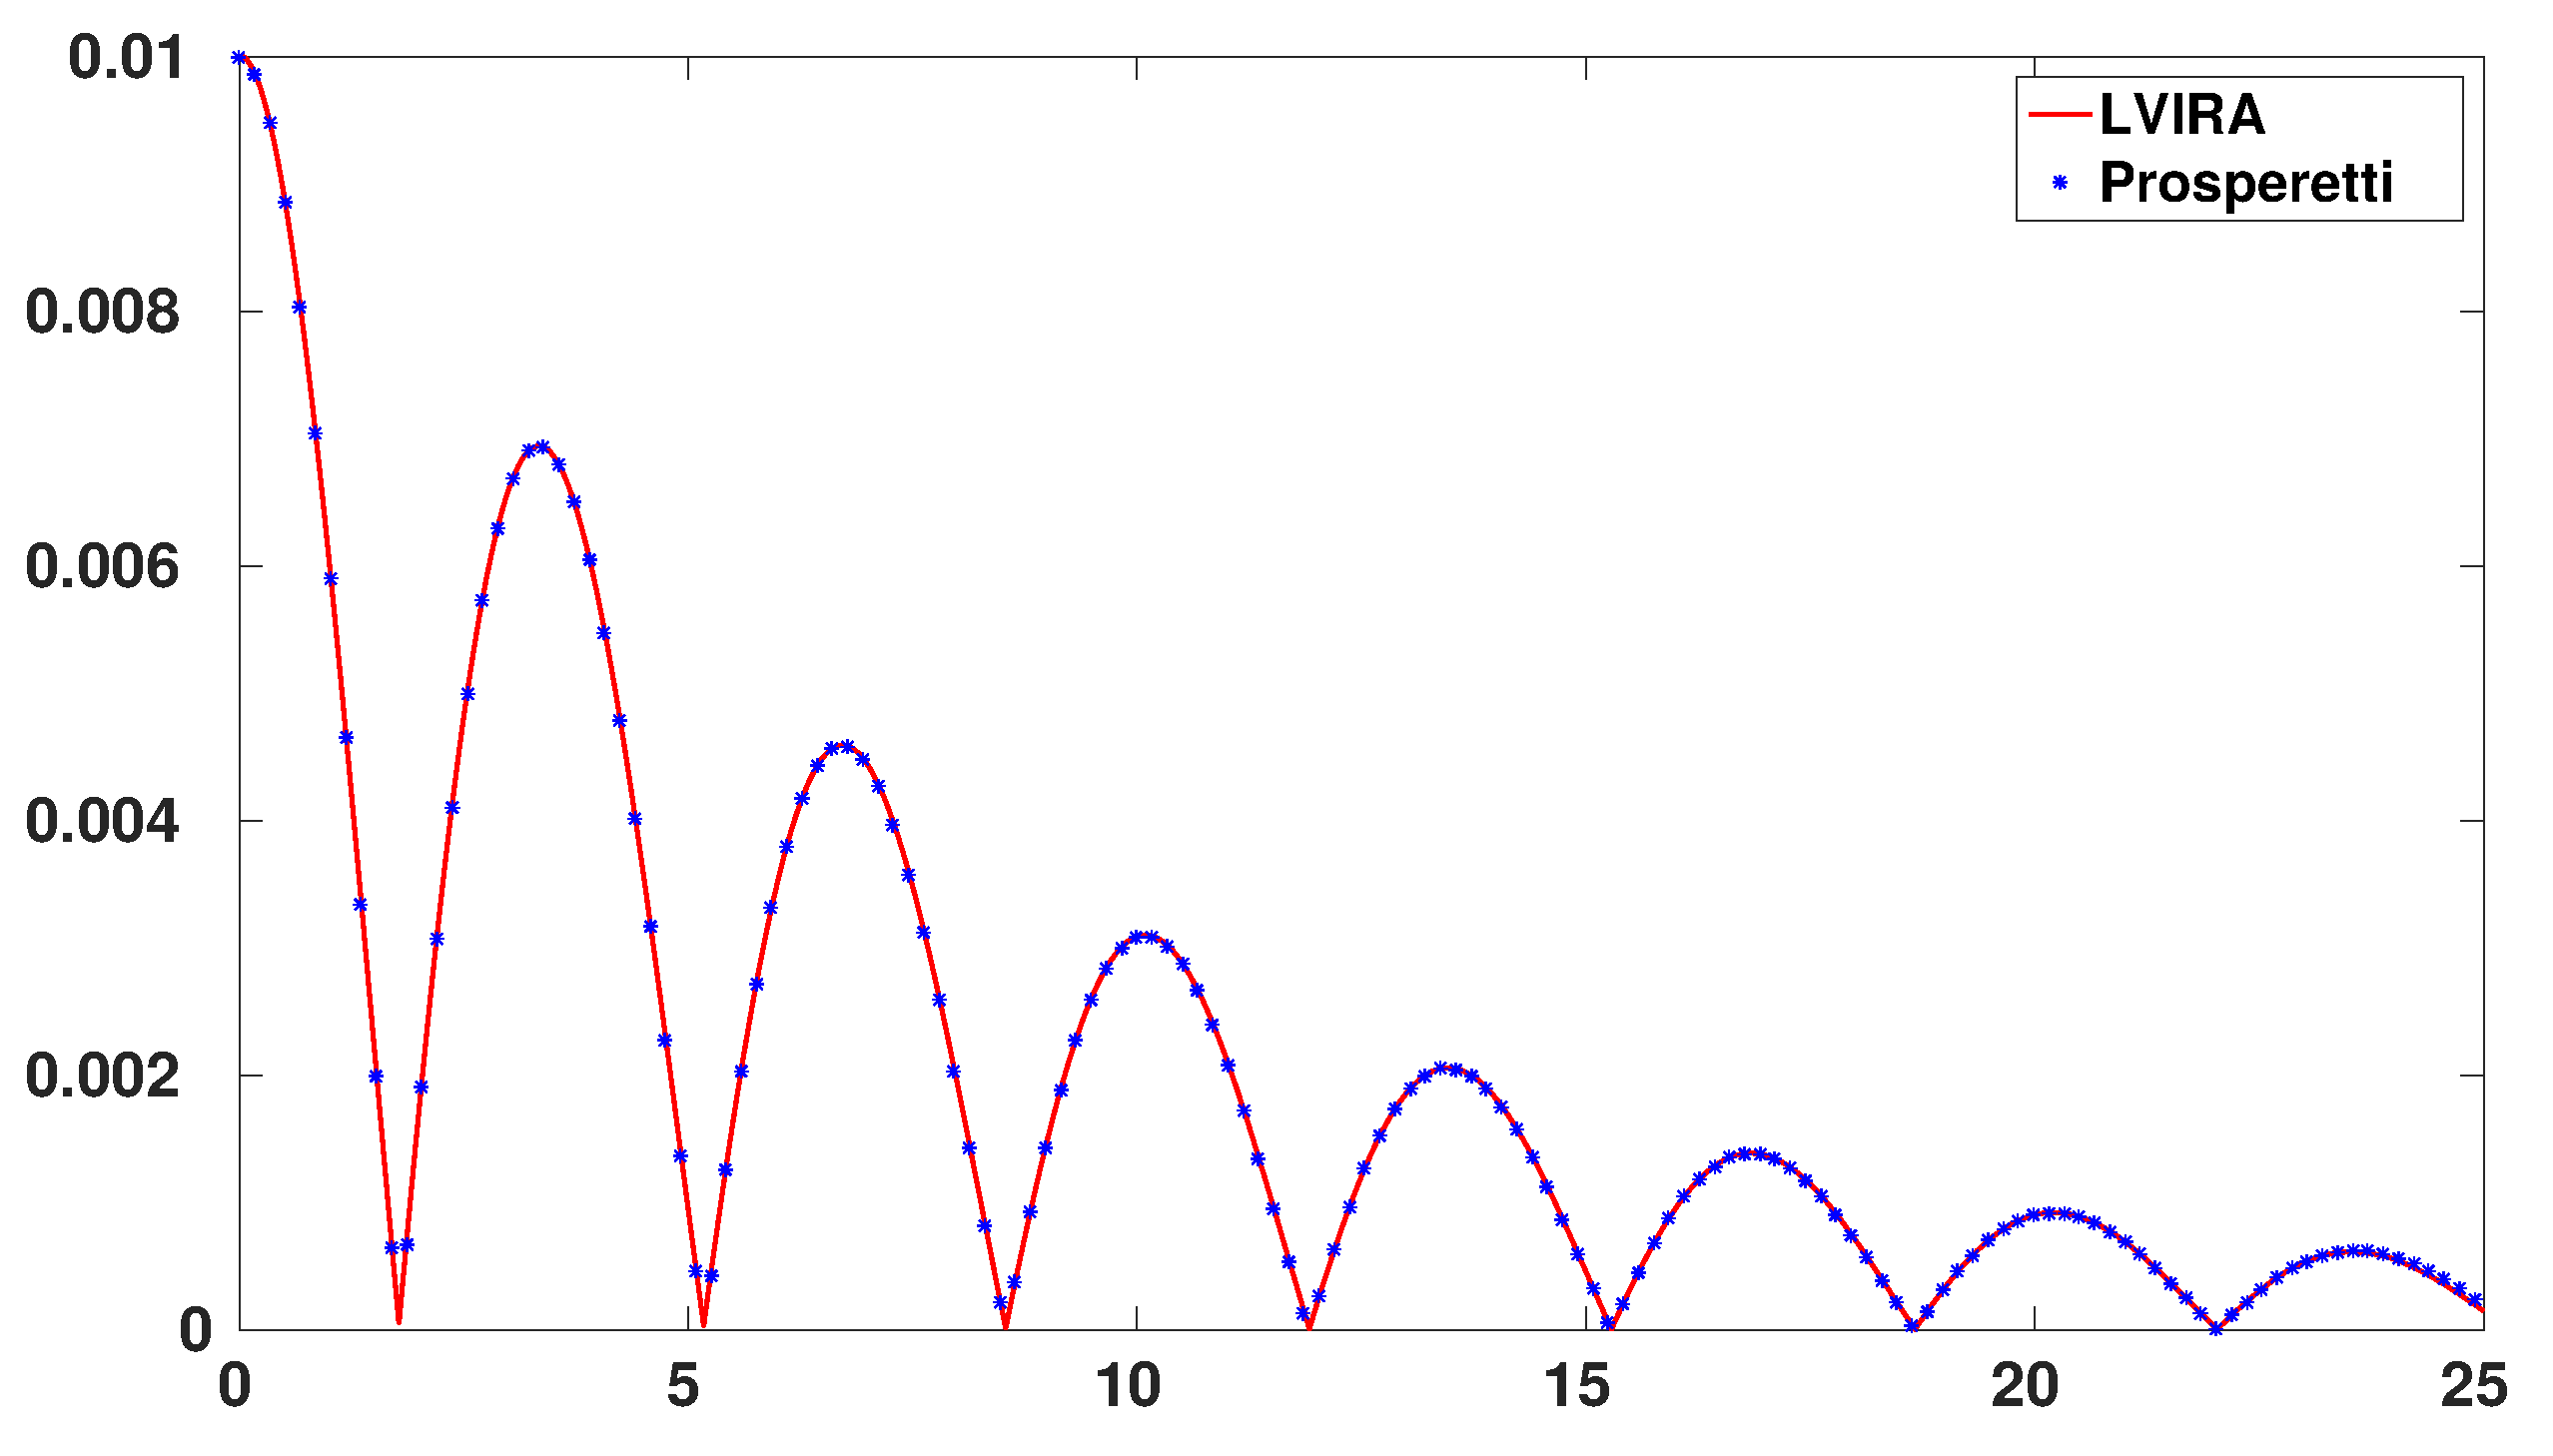
\includegraphics[scale=0.4]{capillary_wave_prosperetti.eps}
 \caption{Comparison with analytical results}
\end{figure}

 